\chapter{Análise Municipal}
\label{cap:sp}

\lettrine{A}{} análise do atendimento das creches da cidade de São Paulo foi baseada na junção dos dados de todos os distritos. A seguir, é mostrado um panorama das matrículas e da demanda ao longo dos 12 anos analisado.

A \autoref{fig:saopaulo} mostra a evolução do atendimento no município.

\begin{figure}[H]
	\centering
	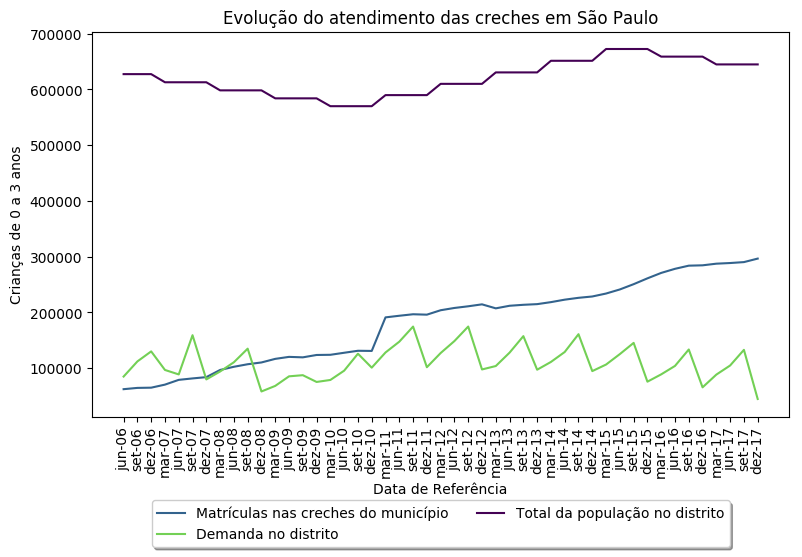
\includegraphics[width=0.7\linewidth]{../Analises/graficos/sao_paulo}
	\caption{Evolução das matrículas, da demanda, e da população de 0 a 3 anos no município de São Paulo.}
	\label{fig:saopaulo}
\end{figure}

É possível notar que existe uma sazonalidade na fila. Ela aumenta durante o ano e cai em dezembro. Nesse mês, parte dos alunos deixa as creches. Com isso, crianças deixam a fila e tornam-se matriculados.

Observa-se também que as matrículas possuem um crescimento constante, menos ao redor de 2010, quando a rede conveniada passou a ser contada. 

Além disso, somando as matrículas com a demanda, percebe-se esse número não chega a 100\% da população de 0 a 3 anos. Isso ocorre porque parte dessa população fica na própria casa com os pais ou com outros familiares, já que a matrícula em creches não é obrigatória.

Para evidenciar que o atendimento melhorou no município como um todo, podem ser analisados o primeiro dado, de junho de 2006 e o último dado, de dezembro de 2017, na \autoref{tab:saopaulo}.

Pode-se observar que o número absurdo de matrículas no fim de 2017 é em torno de 5 vezes maior do que era no meio de 2006. O atendimento chegou a $ 45,93\% $ da população nessa faixa etária. Além disso, nota-se no gráfico que o número de matrículas tende a crescer.

\begin{table}[H]
	\begin{tabular}{|l|l|l|l|}
		\hline
		\textbf{}                                 & \textbf{junho de 2006} & \textbf{dezembro de 2017} & \textbf{Variação} \\ \hline
		\textbf{Número de matrículas}             & 61729                  & 296260                    & +379,94\%       \\ \hline
		\textbf{Crianças na fila}                 & 84408                  & 44092                     & -47,76\%        \\ \hline
		\textbf{População de 0 a 3 anos estimada} & 627552                 & 644996                    & +2,78\%         \\ \hline
		\textbf{Matrículas relativas à população} & 9,84\%              & 45,93\%               & +366,77\%       \\ \hline
		\textbf{Fila relativa à população}        & 13,45\%             & 6,84\%                 & -49,14\%        \\ \hline
	\end{tabular}
	\caption{Comparação do primeiro período com o último analisado.}
	\label{tab:saopaulo}
\end{table}

O dado referente à fila induz a um erro de interpretação. Embora o objetivo dessa parte da análise seja comparar a primeira coleta de dados com a última, é injusto comparar a demanda em diferentes épocas do ano, por causa da sazonalidade associada a ela.

O ideal é comparar a demanda amostrada no mesmo mês do ano. A \autoref{tab:demanda} exibe a informação que permite uma boa análise.

\begin{table}[H]
	\begin{tabular}{|l|l|l|l|}
		\hline
		\textbf{}                                 & \textbf{dezembro de 2006} & \textbf{dezembro de 2017} & \textbf{Variação} \\ \hline
		\textbf{Crianças na fila}                 & 129594                    & 44092                     & -65,98\%       \\ \hline
		\textbf{População de 0 a 3 anos estimada} & 627552                    & 644996                    & +2,78\%        \\ \hline
		\textbf{Fila relativa à população}        & 20,65\%               & 6,84\%                  & -66,88\%        \\ \hline
	\end{tabular}
	\caption{Comparação da demanda no mês de dezembro, em 2006 e 2017.}
	\label{tab:demanda}
\end{table}

Algo ainda a ser observado em relação à fila é que há uma tendência de queda. A sazonalidade atrapalha nessa visualização, mas é possível ver que os picos de mínimo são cada vez menores. Tal tendência é confirmada pelas análises preditivas, exibidas mais à frente.